


\subsection{Results}
Figures~\ref{fig:study1measures} and \ref{fig:study1exp} show the rating scale responses for the seven main subjective measures by condition. 
%
Participants expected the model to improve, and they expected more improvement with feedback. Participants also thought the ability to provide feedback was important. 
%
Explanations hurt subjective satisfaction (frustration, trust, and acceptance ratings), while feedback helped.
%
Participants were commonly frustrated by the model's low quality, and this was accentuated by explanations. 

To judge user comfort with the task and dataset, we asked participants to tell us (i.e., the researchers \dots not the model) whether they thought each email was about hockey, baseball, or whether they were unsure.
%
Participants did well: 91\% of the 3,580 answers reported to us were correct, while 8\% were ``not sure'' and only 1\% were incorrect. In the following sections, we provide detailed results regarding satisfaction, expectations, perceptions, feedback quality, and users' desire to provide feedback.

\begin{figure}[t]
    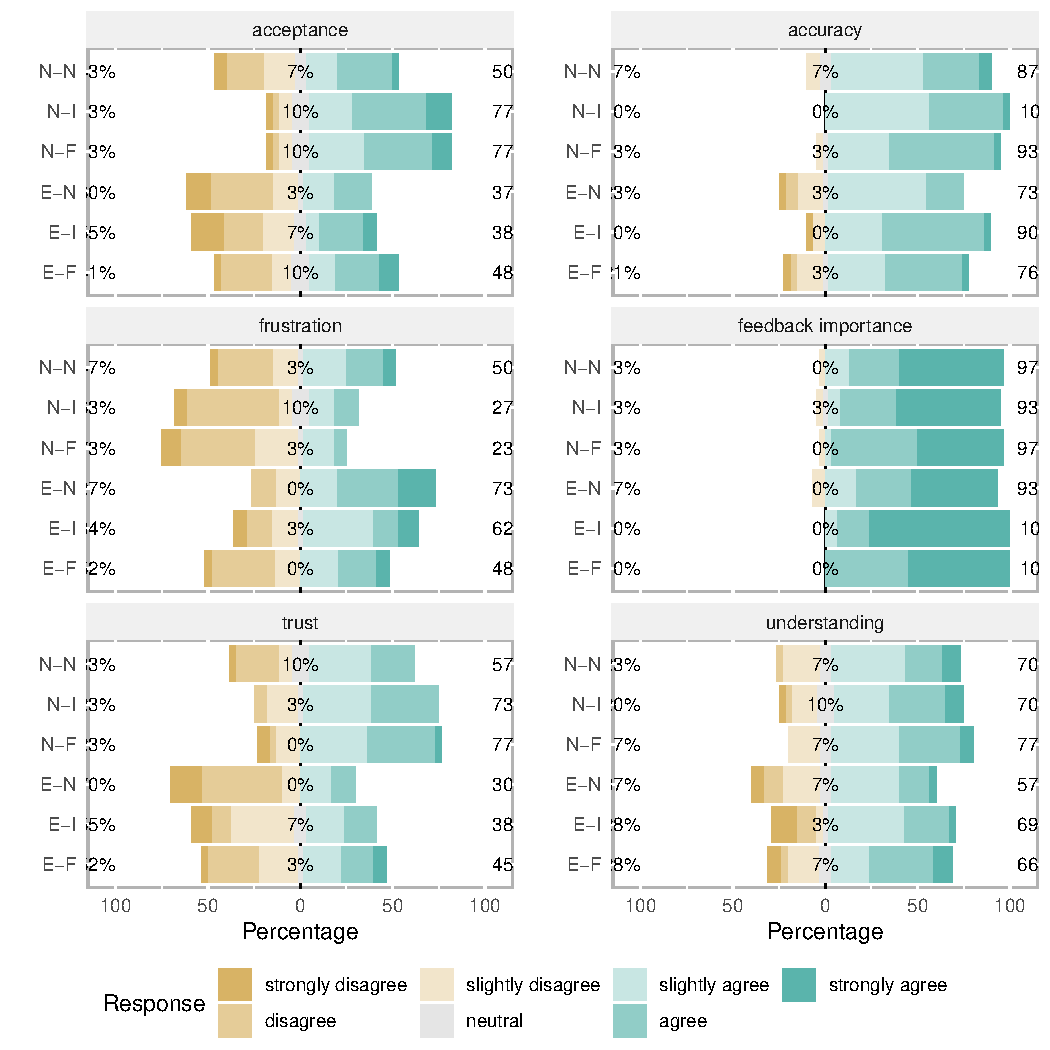
\includegraphics[width=\linewidth]{figures/study1-measures}
    \caption{Study~1 seven-point rating scale responses for the main subjective measures (except expected change) from ``strongly disagree'' to
``strongly agree''. Responses reported by condition. For each measure,
no explanation (N-) conditions are on the top (-N is with no feedback, -I
is with instance-level feedback, and -F is with feature-level feedback) and
feature explanation (E-) conditions are below Feedback (-I, -F) positively,
and explanation (E-) negatively impact satisfaction measures (left).}
\label{fig:study1measures}
\end{figure}

\subsubsection{User Satisfaction}
% four points: frustration measure, why frustrated, trust, acceptance
Participants were neutral on average, but with high variability across conditions, for each of the user satisfaction measures: frustration ($M=3.9$ of 7, $SD=1.8$), trust ($M=4.1, SD=1.7$), and whether they would use the system (acceptance) ($M=4.3, SD=1.9$).
%
Feedback significantly improved satisfaction, but explanations hampered it. Open-ended responses suggested that the low model quality---highlighted by explanations---frustrated participants.

\textbf{Explanations increased frustration, while support for feedback reduced it}. 
%
Participants who received explanations were more frustrated than those who did not; this difference was significant (main effect of \textit{Explanation}: $F_{1, 172}=20.05, p < .001$). \textit{Feedback} also significantly impacted frustration (main effect: $F_{2, 172}=7.92, p < .001$). Posthoc pairwise comparisons showed that no feedback resulted in significantly higher frustration than instance-level and feature-level feedback (both comparisons $p<.05$); this supports \textbf{H1.1} for frustration, which stated that feedback would reduce frustration. The interaction between \textit{Explanation} and \textit{Feedback} was not significant ($F_{2, 172}=.06, p=.094$); thus, \textbf{H1.2} is only partially supported by the main effect of \textit{Feedback}. 

% why frustrated
\textbf{Many participants were frustrated by low quality, which was highlighted by explanations}.
%
We coded participants' open-ended reasons for their frustration ratings, resulting in six codes. Participants felt the model was: ``not good enough'' ($40\%$ of the 178), or ``good enough'' ($27\%$), would help ``save time'' ($13\%$), would ``require user review'' of the decisions ($11\%$), is ``able to improve'' ($3\%$), or ``other'' reasons ($6\%$).

Confirming the rating scale data, more participants with explanations ($81\%$ of 89) thought the model was ``not good enough'' compared to those who did not get explanations (only $26\%$ of 89).
%
Participants who got explanations (E-) often expressed their frustration in terms of the important words, e.g., \textit{``I don't think it highlighted the best words in many cases''} (LP3, E-I), while those who did not see explanations (N-) were more likely to comment on the model's shortcomings in terms of accuracy, \textit{``it made too many mistakes''} (LP175, N-N). 
%
%``Requires user review'' was a similar concern mentioned by 11\% of all 179 participants, such as \textit{``it would take longer to do my job because I would have to check for accuracy''} (LP151, E-I).

Less frustrated participants felt the model was ``good enough'' or would ``save time'', saying, for example, %\textit{``this model appears to sort the emails with an acceptable degree of accuracy''} (LP52 N-F) and, 
\textit{``It would be much easier than sorting through them myself''} LP132 (E-N).
%Demonstrating lower frustration, 27\% of all participants felt the model was ``good enough,'' such as, \textit{``this model appears to sort the emails with an acceptable degree of accuracy''} (LP52, N-F), and 13\% thought that it would ``save time,'' such as, \textit{``It would be much easier than sorting through them myself''} (LP132, E-N).

% trust measure
\textbf{Trust and acceptance were reduced by explanations and increased by feedback}.
%
Reflecting the frustration findings, trust was significantly impacted by \textit{Explanation} ($F_{1, 172}=14.57, p < .001$); participants who received explanations trusted the model less those who did not. There was also a significant main effect of \textit{Feedback} on trust ($F_{2, 172}=4.27, p = .015$). Posthoc pairwise comparisons showed that both instance- and feature-level feedback increased trust compared to none (both comparisons $p<.05$). The \textit{Explanation} $\times$ \textit{Feedback} interaction was not significant ($F_{2, 172}=.15, p=.863$).

Similarly, \textit{Explanation} significantly impacted acceptance ($F_{1, 172}=19.49, p < .001$), where participants who saw explanations accepted the model less than those who did not. 
\textit{Feedback} also significantly impacted acceptance ($F_{2, 172}=3.76, p=.025$). Posthoc pairwise comparisons showed that feature-level feedback resulted in higher model acceptance compared to none ($p<.05$). The interaction between \textit{Explanation} and \textit{Feedback} was not significant ($F_{2, 172}=.97, p=.38$).


\subsubsection{User Expectations for and Perceptions of the Model}
% expectation of improvement and why, understanding, accuracy
Participants provided subjective ratings of their perceptions and expectations (Figure~\ref{fig:study1measures} and~\ref{fig:study1exp}).
On average, they expected the model to improve ($M=5.2, SD=.9$), thought it worked fairly well ($M=5.2$, $SD=1.1$), and were neutral regarding whether they understood how it works ($M=4.7$, $SD=1.6$). 
%
We also examined expectations through participants' \textit{simulated model predictions}: how they thought the model would label the four evaluation emails at the end of the study. %---emails that were the same or similar to ones that had been shown in the earlier set of 20. %A substantial portion of participants expect the model to improve, even those that did not provide feedback to it; we see this in both the subjective ratings and simulated model predictions. Participants' open-ended reasons for their expected improvement ratings suggest some think ML models may \textit{self correct} from mistakes.   
As detailed below, feedback caused participants to think the model was more accurate and would improve, but explanation did not. Moreover, some participants who did not provide feedback thought the model would \textit{self-correct}.

%For each email type (same or similar), we included one that the model previously predicted incorrectly and one for which it was previously correct.\lkf{this description is clearer than it was earlier in the protocol. Could maybe cut this last sentence here though.}

\begin{figure}
    \centering
    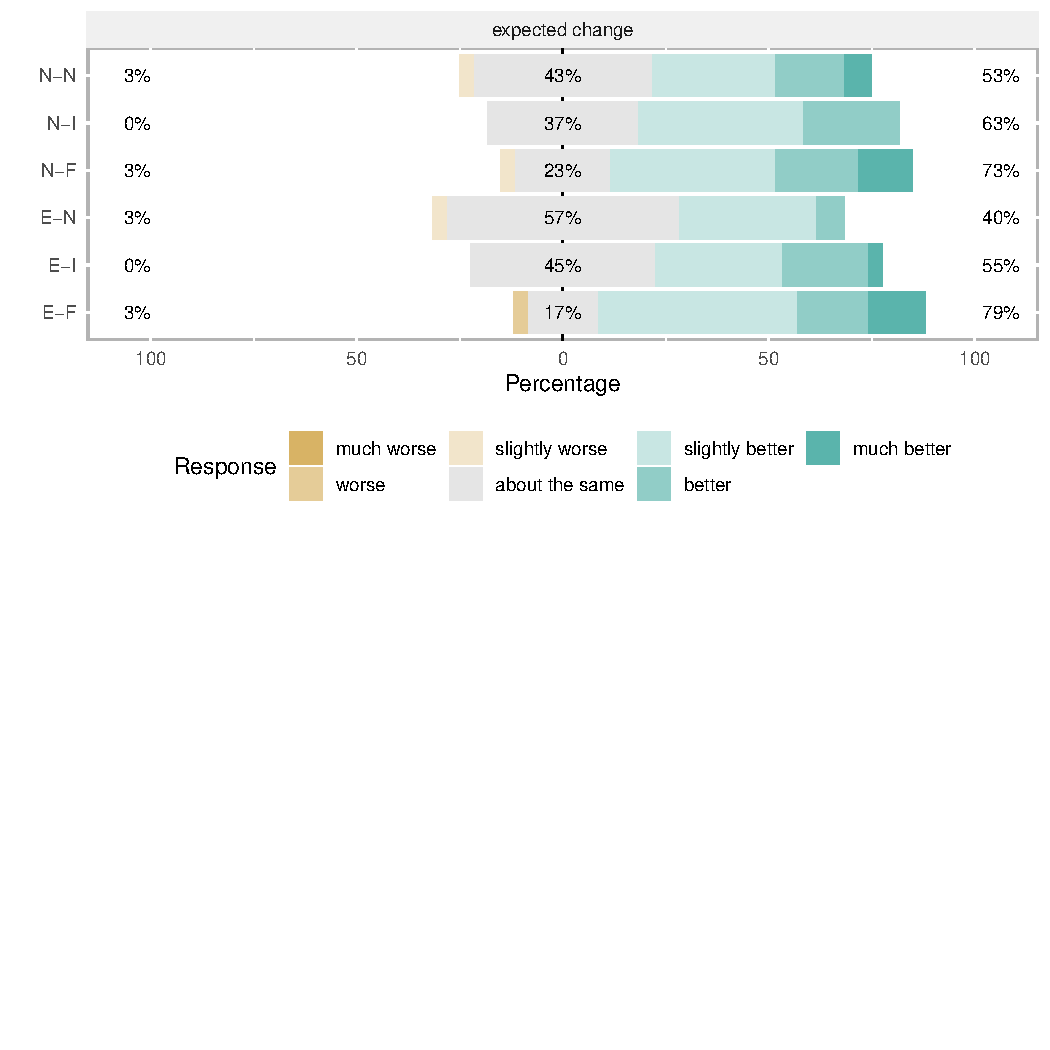
\includegraphics[width=\linewidth]{figures/exp-plots-study1.pdf}
    \caption{Study 1 participant responses for the subjective expected
change measure by condition. Participants expected
the model to improve. (Figure~\ref{fig:study1measures} describes $y$-axis labels.)}
    \label{fig:study1measures}
\end{figure}

\textbf{Feature-level feedback increased expected improvement compared to no feedback}.
%
\textit{Feedback} significantly increased users' expectations ($F_{2,172}=5.29, p=.006$);  post-hoc comparisons showed that feature-level feedback raised expected improvement compared to no feedback ($p<.05$), partially supporting \textbf{H2.1}. The main effect of \textit{Explanation} was not significant ($F_{1,172}=1.28, p=.259$; opposing \textbf{H2.2}), nor was the \textit{Explanation} $\times$ \textit{Feedback} interaction ($F_{2,172}=.42, p=.656$).

\textbf{A substantial portion of participants expected model corrections, even without feedback}.
%
Across all three feedback conditions, about half or more of participants expected the model to improve (rating > 4): 76.3\% of 59 who had feature-level feedback, 59.3\% of 59 who had instance-level feedback, and even $47\%$ of 60 who had no feedback. 

%Confirming our rating scale data, of the 118 participants who provided feedback, more expected model improvement after giving feature-level feedback (45 of 59) than those that provided instance-level feedback (35 of 59).
%Of the 60 participants who did not provide feedback, $53\%$ (of 30) who did not receive an explanation and $40\%$ (of 30) who did thought the model would improve. Suggesting that explanations tempered expected improvement in the no feedback condition.

%After the interaction phase, participants predicted how the model would ``now'' label emails that were the same as or similar to emails in the original set of 20. 
Participants' predictions about how what the model would do with the four same/similar ``evaluation'' emails  reflected this strong expectation of improvement. 
%, resulting in 712 \textit{simulated model predictions}. 
For the previously correct emails, participants thought the model would now be incorrect in only 4 of 712 instances, and each of these was for a ``similar'' email rather than the email that was exactly the ``same'' as in the initial set of 20.

For the previously incorrect emails, ``similar'' and ``same'' follow a similar pattern, so we focus on the ``same'' email to provide a straightforward assessment of whether participants think the model will improve. 
%
Most (82\%) of participants who provided feedback ($N=118$) thought the model would get the previously incorrect email correct (Table~\ref{tab:study1eval}), which is not surprising given that they had spent time trying to improve the model.
%
More surprising, however, is that 53\% of  participants in the no feedback condition ($N=60$) thought the model would somehow correct itself. %As with the subjective rating scale data, Table~\ref{tab:study1eval} shows that the influence of explanations on this expectation for improvement is, if anything, unclear.

\begin{table}[t]
    \centering
    \begin{tabular}{cccc}
    \toprule
              & \multicolumn{3}{c}{{\bf Feedback}} \\
              \cline{2-4}
        {\bf Explanation} & None & Instance & Feature \\
         \midrule
        None & 63\% & 80\% & 90\% \\
        Feature & 43\% & 86\% & 73\% \\
        \bottomrule
    \end{tabular}
    \caption{Percentage of Study 1 participants (\textit{N}=178) by condition during the ``evaluation phase'' who thought the model would now correctly label an email it had previously labeled incorrectly. Many participants in the \textit{no feedback} conditions thought the model would self correct.}
    \label{tab:study1eval}
    \vspace{-15pt}
\end{table}

\textbf{Participants described the model improving from their feedback or learning from its mistakes}.
We coded participants open-ended reasons for their expected change ratings, resulting in nine codes. Participants felt the model would improve with ``feedback'' ($29\%$), was capable of ``self learning'' ($20\%$), was ``high quality'' ($5\%$), or showed ``evidence of improvement'' ($1\%$). 
%
Those who felt it would not improve cited that it received ``inadequate feedback'' ($14\%$), showed ``no evidence of improvement'' ($11\%$), had ``nothing to learn from'' ($6\%$) or was of ``low quality'' ($5\%$). And, $9\%$ of participants gave ``other'' reasons.
%
%Many participants expected the model to improve from the ``feedback'' they provided (29\% of all 178 participants) or that it would \textit{self correct} (i.e., model ``self learning'' from its mistakes) (20\%). 

Interestingly, of the 60 participants who did not provide feedback (-N), 17 (28\%) still expected the model to learn from its mistakes, such as,  \textit{``it would take what it did wrong, learn from it, and apply it in future trials''} (LP141, N-N), or reported other misconceptions, including, \textit{``these programs get better as they function and learn algorithms''} (LP154, E-N). 
%
In fact, only 13\% of the 60 participants who did not provide feedback \textit{correctly} identified that the model would not improve as it had ``nothing to learn from'', like, \textit{``if it still used the same words to try to identify the correct sports emails, then it would still make the same amount of errors''} (LP87, E-N).

%Twenty-one participants (12\%) thought they provided ``inadequate feedback'', or not enough (quality or quantity) to improve the model. \lkf{is the rest of this para interesting or can we cut it}10 of these gave instance-level feedback (6 provided feature-level and 5 provided no feedback) and suggested the model needed additional information beyond just labels, such as keywords. For example, LP60 (E-I) said, \textit{``It would have been better if I'd had the option to tell it when it should have looked at different keywords''}, while LP72 (E-I) said, \textit{``I don't know what it learned, because I wasn't able to provide detailed feedback''}.
%Of the 21 participants who thought the system was given ``inadequate feedback, 10 gave instance-level feedback and suggested the model needed additional information beyond just labels, such as keywords. For example, LP60 (E-I) said, \textit{``It would have been better if I'd had the option to tell it when it should have looked at different keywords''}, while LP72 (E-I) said, \textit{``I don't know what it learned, because I wasn't able to provide detailed feedback''}. 

%Finally, some participants were not sure if the model would improve as there was ``no evidence of improvement'' during the interaction phase. $11\%$ of all participants suggested this, and surprisingly, $15\%$ of the 118 participants who gave feedback reported this, even though we explicitly reminded those participants that the model would not update with their feedback until after the interaction phase.\lkf{this last sentence is similar to the findings already reported in the prev improvement section, again suggesting to me that you should put this qual stuff up there and shorten it}

\textbf{Feature-level feedback reduced perceived accuracy compared to no feedback}.
%
\lkf{this is weird and needs to be touched on in Discussion}
Overall, participants thought the system worked fairly well, giving it an average accuracy rating across all conditions of 5.2 out of 7 ($SD=1.1$).
However, counter to our other user experience measures, feature-level feedback had a negative effect on perceived accuracy. There was a significant main effect of \textit{Feedback} on perceived accuracy ($F_{2,172}=4.72, p=.010$), with posthoc pairwise comparisons showing that feature-level feedback reduced perceived accuracy compared to no feedback ($p<.05$). Neither the main effect of \textit{Explanation} nor the \textit{Explanation} $\times$ \textit{Feedback} interaction effect were significant (respectively: $F_{1,172}=1.59, p=.209$; $F_{2,172}=2.20, p=.114$). 

\subsubsection{Quality of and Desire for User Feedback}
% three points: users want to provide feedback, how good is their feedback for the model, and how do users 'features' compare to the model's 'features'
Participants thought being able to provide feedback was important ($M=6.4$ out of 7, $SD=.9$), regardless of condition~(Figure~\ref{fig:study1measures}); there were no significant main or interaction effects on this measure. However, do the experimental conditions impact feedback \textit{quality}? To answer this question, we applied participants' feedback to the model after the study.

\textbf{Feedback improved the model, regardless of explanation}.
%, and explanation does not appear to impact this improvement}.
We incorporated instance-level feedback by including the 20 emails labeled by the participant as additional training emails. To incorporate the feature-level feedback, we adjusted the classifier's weight for each word provided by the participant: the word weight was both increased by 20\% for the specified class and decreased by 20\% for the opposite class.\lkf{seems arbitrary... anything we can cite here a way we can justify?}\amr{agreed... Ron or Melissa?}\jbg{If it was $\beta_a \rightarrow \frac{\beta_a + \alpha_a}{\sum \beta_\cdot + \alpha_a}$, then you can phrase it as increasing the Dirichlet prior with a $\beta$ pseudocount (i.e., the user provided an additional training example with weight $\alpha$; this is how Settles justified it).}
%This resulted in $59$ feature-updated models and $59$ instance-updated models.

The feature-updated models were 86.2\% accurate on average ($SD=2.7\%$), which is a 9.7 percentage point improvement over the initial low quality model.
In comparison, the instance-updated models were 83.6\% accurate ($SD=1.4\%$)---a 7.1 percentage point improvement. Instance and feature model improvements were similar regardless of whether the participants saw an explanation (difference in accuracy $<.2\%$).

\textbf{Participants did not agree with the words the model thought were important}.
The 59 participants who gave feature-level feedback highlighted a total of $3,533$ words. Regardless of whether explanations were shown or not, we compared the model's top three words for each email (i.e., the words the model would have highlighted) to the three words selected by the participant. Most (76.9\%) of the participants' words were not in the model's top set. This disagreement is likely due both to the model's low quality and because the explanation method can highlight words that are probable for the non-predicted class (see Limitations). Participants with explanations were more likely to reuse the model's words (28\% of selected words overlapped with the model's) than the 30 participants who did not see explanations (21\%).  

\subsection{Summary}
Explanations significantly increased frustration, while feedback---especially feature-level---significantly decreased it (partial support for \textbf{H1.1} and \textbf{H1.2}). There were similar patterns for other user satisfaction measures (trust and acceptance). Therefore, the worst combination was explanation without feedback, and the best was no explanation with feedback. Open-ended responses suggested that frustration was primarily due to the low model quality exposed by explanations and \textit{not} inability to provide feedback, as we had hypothesized. Although ability to provide feedback did temper some of the frustration. This general dislike for explanations confirms prior work where user perceptions were negatively impacted by explanations that exposed flaws and limitations~\cite{Cai2019TheInterface}. While this may seem inconsistent with our hypothesis at first blush, an alternate interpretation is that explanations can improve satisfaction \emph{so long as users have a means for feedback}. 

Feedback also significantly increased expectations of model improvement, as hypothesized in \textbf{H2.1}, but particularly for feature-level feedback opposed to none. Explanation did not impact expected change, in contrast to \textbf{H2.2}.
Also, somewhat surprisingly, participants  expected the model to improve; including many who had not provided feedback. %We discuss this and general misconceptions regarding ML models in the Discussion.
